\section{Mathematical Uncertainty Theories}

As mentioned in \cite{uncertaintymeasuresbigpicture} and further detailed in chapters 2 and 3 of \cite{UncertaintySciences}, a theory of uncertainty typically consists of two elements:

\begin{romanenum}
    \item A mathematical representation that encodes data about uncertain states of the world.
    \item Mathematical operators and measures that enable reasoning about and combining uncertain information.
\end{romanenum}

As shown in Figure \ref{fig:Generalized_sets}, data is encoded via different generalizations of sets, according to what is considered precise or not (elements and sets). These set models are examples of theories that tackle a specific representation, but are not the only possible models.\\

When choosing a proper model for a concrete problem, one should 
take into account that the more expressive and general a framework 
is, the more complicated it becomes due to all the nuances it 
attempts to capture. Therefore, if precise information is 
available, it should not be treated as imprecise. For this reason, precise information should be modeled as precise rather than imprecise when available. This trade-off will be explored further in our discussion of possibilities versus probabilities, where possibilities offer greater expressiveness but lower predictive power.


\begin{figure}[ht]
    \hspace{2cm}
    \begin{tikzpicture}[>=stealth, font=\sffamily, align=center]
        % Define column x-positions.
        \def\xOne{-3}   % Column 1: Elements of Universal Set
        \def\xTwo{0}    % Column 2: Set (or event as a notion)
        \def\xThree{3}  % Column 3: Set Membership
        \def\xFour{6}   % Column 4: Example Theories
        
        % Use a common vertical center (here chosen as 0).
        \def\Bgap{0.75}
        
        % Column 2 vertical shifts.
        \def\CshiftA{2.25}
        \def\CshiftB{0.75}
        \def\CshiftC{-0.75}
        \def\CshiftD{-2.25}
        
        % Column 3 and Column 4 vertical shifts.
        \def\Dshiftone{5.25}
        \def\Dshifttwo{3.75}
        \def\Dshiftthree{2.25}
        \def\Dshiftfour{0.75}
        \def\Dshiftfive{-0.75}
        \def\Dshiftsix{-2.25}
        \def\Dshiftseven{-3.75}
        \def\Dshifteight{-5.25}
        
        % --------------------- Column 1 ---------------------
        % Small nodes
        \node (B1) at (\xOne, \Bgap)
              [rectangle, draw, fill=blue!10] {Precise\\ elements};
        \node (B2) at (\xOne, -\Bgap)
              [rectangle, draw, fill=blue!10] {Imprecise\\ elements};
              
        % Big rectangle in the background layer
        \begin{pgfonlayer}{background}
        \node[draw, thick, rounded corners,
              fill=gray!10,
              fit=(B1)(B2),
              inner sep=5pt,
              label={[align=center]above:\textbf{Elements}}
        ] (BoxB) {};
        \end{pgfonlayer}
        
        % --------------------- Column 2 ---------------------
        \node (C1) at (\xTwo, \CshiftA)
              [rectangle, draw, fill=blue!10] {Precise\\ set};
        \node (C2) at (\xTwo, \CshiftB)
              [rectangle, draw, fill=blue!10] {Imprecise\\ set};
        \node (C3) at (\xTwo, \CshiftC)
              [rectangle, draw, fill=blue!10] {Precise\\ set};
        \node (C4) at (\xTwo, \CshiftD)
              [rectangle, draw, fill=blue!10] {Imprecise\\ set};
        
        \begin{pgfonlayer}{background}
        \node[draw, thick, rounded corners,
              fill=gray!10,
              fit=(C1)(C4),
              inner sep=5pt,
              label={[align=center]above:\textbf{Set}}
        ] (BoxC) {};
        \end{pgfonlayer}
        
        % --------------------- Column 3 ---------------------
        \node (D1) at (\xThree, \Dshiftone)
              [rectangle, draw, fill=blue!10] {Binary};
        \node (D2) at (\xThree, \Dshifttwo)
              [rectangle, draw, fill=blue!10] {Non-\\binary};
        \node (D3) at (\xThree, \Dshiftthree)
              [rectangle, draw, fill=blue!10] {Binary};
        \node (D4) at (\xThree, \Dshiftfour)
              [rectangle, draw, fill=blue!10] {Non-\\binary};
        \node (D5) at (\xThree, \Dshiftfive)
              [rectangle, draw, fill=blue!10] {Binary};
        \node (D6) at (\xThree, \Dshiftsix)
              [rectangle, draw, fill=blue!10] {Non-\\binary};
        \node (D7) at (\xThree, \Dshiftseven)
              [rectangle, draw, fill=blue!10] {Binary};
        \node (D8) at (\xThree, \Dshifteight)
              [rectangle, draw, fill=blue!10] {Non-\\binary};
        
        \begin{pgfonlayer}{background}
        \node[draw, thick, rounded corners,
              fill=gray!10,
              fit=(D1)(D8),
              inner sep=5pt,
              label={[align=center]above:\textbf{Set Membership}}
        ] (BoxD) {};
        \end{pgfonlayer}
        
        % --------------------- Column 4 ---------------------
        \node (E1) at (\xFour, \Dshiftone)
              [rectangle, draw, fill=blue!10] {Crisp\\ sets};
        \node (E2) at (\xFour, \Dshifttwo)
              [rectangle, draw, fill=blue!10] {Rough\\ sets};
        \node (E3) at (\xFour, \Dshiftthree)
              [rectangle, draw, fill=blue!10] {Illogical};
        \node (E4) at (\xFour, \Dshiftfour)
              [rectangle, draw, fill=blue!10] {Fuzzy\\ sets};
        \node (E5) at (\xFour, \Dshiftfive)
              [rectangle, draw, fill=blue!10] {Illogical};
        \node (E6) at (\xFour, \Dshiftsix)
              [rectangle, draw, fill=blue!10] {Fuzzy\\ rough sets};
        \node (E7) at (\xFour, \Dshiftseven)
              [rectangle, draw, fill=blue!10] {Illogical};
        \node (E8) at (\xFour, \Dshifteight)
              [rectangle, draw, fill=blue!10] {Rough\\ fuzzy sets};
        
        \begin{pgfonlayer}{background}
        \node[draw, thick, rounded corners,
              fill=gray!10,
              fit=(E1)(E8),
              inner sep=5pt,
              label={[align=center]above:\textbf{Set Models}}
        ] (BoxE) {};
        \end{pgfonlayer}
        
        % --------------------- Edges ---------------------
        % Column 1 -> Column 2:
        \draw[->] (B1) to[bend right=10] (C1);
        \draw[->] (B1) to[bend left=10] (C2);
        \draw[->] (B2) to[bend right=10] (C3);
        \draw[->] (B2) to[bend left=10] (C4);
        
        % Column 2 -> Column 3:
        \draw[->] (C1) to[bend right=10] (D1);
        \draw[->] (C1) to[bend left=10] (D2);
        \draw[->] (C2) to[bend right=10] (D3);
        \draw[->] (C2) to[bend left=10] (D4);
        \draw[->] (C3) to[bend right=10] (D5);
        \draw[->] (C3) to[bend left=10] (D6);
        \draw[->] (C4) to[bend right=10] (D7);
        \draw[->] (C4) to[bend left=10] (D8);
        
        % Column 3 -> Column 4:
        \draw[->] (D1) -- (E1);
        \draw[->] (D2) -- (E2);
        \draw[->] (D3) -- (E3);
        \draw[->] (D4) -- (E4);
        \draw[->] (D5) -- (E5);
        \draw[->] (D6) -- (E6);
        \draw[->] (D7) -- (E7);
        \draw[->] (D8) -- (E8);
        
    \end{tikzpicture}
    \caption{Generalizations of crisp sets with different set models, showing increasing levels of expressivity for encoding data uncertainty. Adapted from Figure 2.1 in \cite{UncertaintySciences}.}
    \label{fig:Generalized_sets}
\end{figure}



Regarding operators and measures (most based on the previous set models), there exist many different frameworks, with varying levels of development and adoption. In Figure \ref{fig:uncertainty_taxonomy}, Cuzzolin \cite{uncertaintymeasuresbigpicture} maps out the major uncertainty theories and notes that \say{The \say{quality} of the various proposals differs radically}. As an example, he points out that Liu's Uncertainty Theory lacks rigorous mathematical foundations and convincing justification. \\

Another interesting observation stated in the paper is that generality isn't the only factor that matters, as the most general frameworks haven't experienced the growth and adoption one might expect. This is likely because overly general frameworks can become intractable and unnecessarily complex without providing clear practical benefits:

\hspace{1cm}\say{Imprecise probability is remarkable for its generality, asspecial cases of coherent lower previsions include probabilities, de Finetti previsions, Choquet capacities, possibility and belief measures, random sets but also probability boxes, (lower and upper envelopes of) credal sets, and robust Bayesian models. Nevertheless, IP has so far failed to achieved the expected impact in both mathematical statistics and application fields. This may lead to the reflection that generality, after all, is not the real thing.}\cite{uncertaintymeasuresbigpicture}\\

The majority of these frameworks emerged to address key limitations of probability theory. Some of these limitations include:
\begin{romanenum}
      \item \textbf{Second-Order Uncertainty:} Probability theory handles risk well but fails to capture uncertainties about the probability model itself.
      \item \textbf{Ignorance Representation:} There is no probability distribution that assigns equal probability to every single event (not even the uniform distribution). There the state of absolute ignorance is not possible.
      \item \textbf{Imprecision in Data:} The additive nature of probability struggles with fuzzy, ambiguous, or set-valued data.
      %\item \textbf{Scarce Data Limitations:} It relies on large datasets, making it less effective when data is incomplete or limited.
      \item \textbf{Additivity Constraint:} The strict additivity axiom prevents modeling non-additive phenomena common in real-world uncertainty.
      %\item \textbf{Update and Combination Challenges:} Bayesian inference requires well-justified priors and often struggles to combine uncertain evidence.
      %\item \textbf{Alternative Reasoning Incompatibility:} It does not integrate smoothly with frameworks like fuzzy logic or belief functions.
      %\item \textbf{Decision-Making Mismatch:} Observed human behavior under uncertainty (e.g., Ellsberg's paradox) often contradicts classical probabilistic predictions.
      \item \textbf{Rigidity in Assumptions:} The need for well-defined sample spaces and distributions is frequently unrealistic in complex, real-world scenarios.
    \end{romanenum}
    




\begin{figure}[ht]
    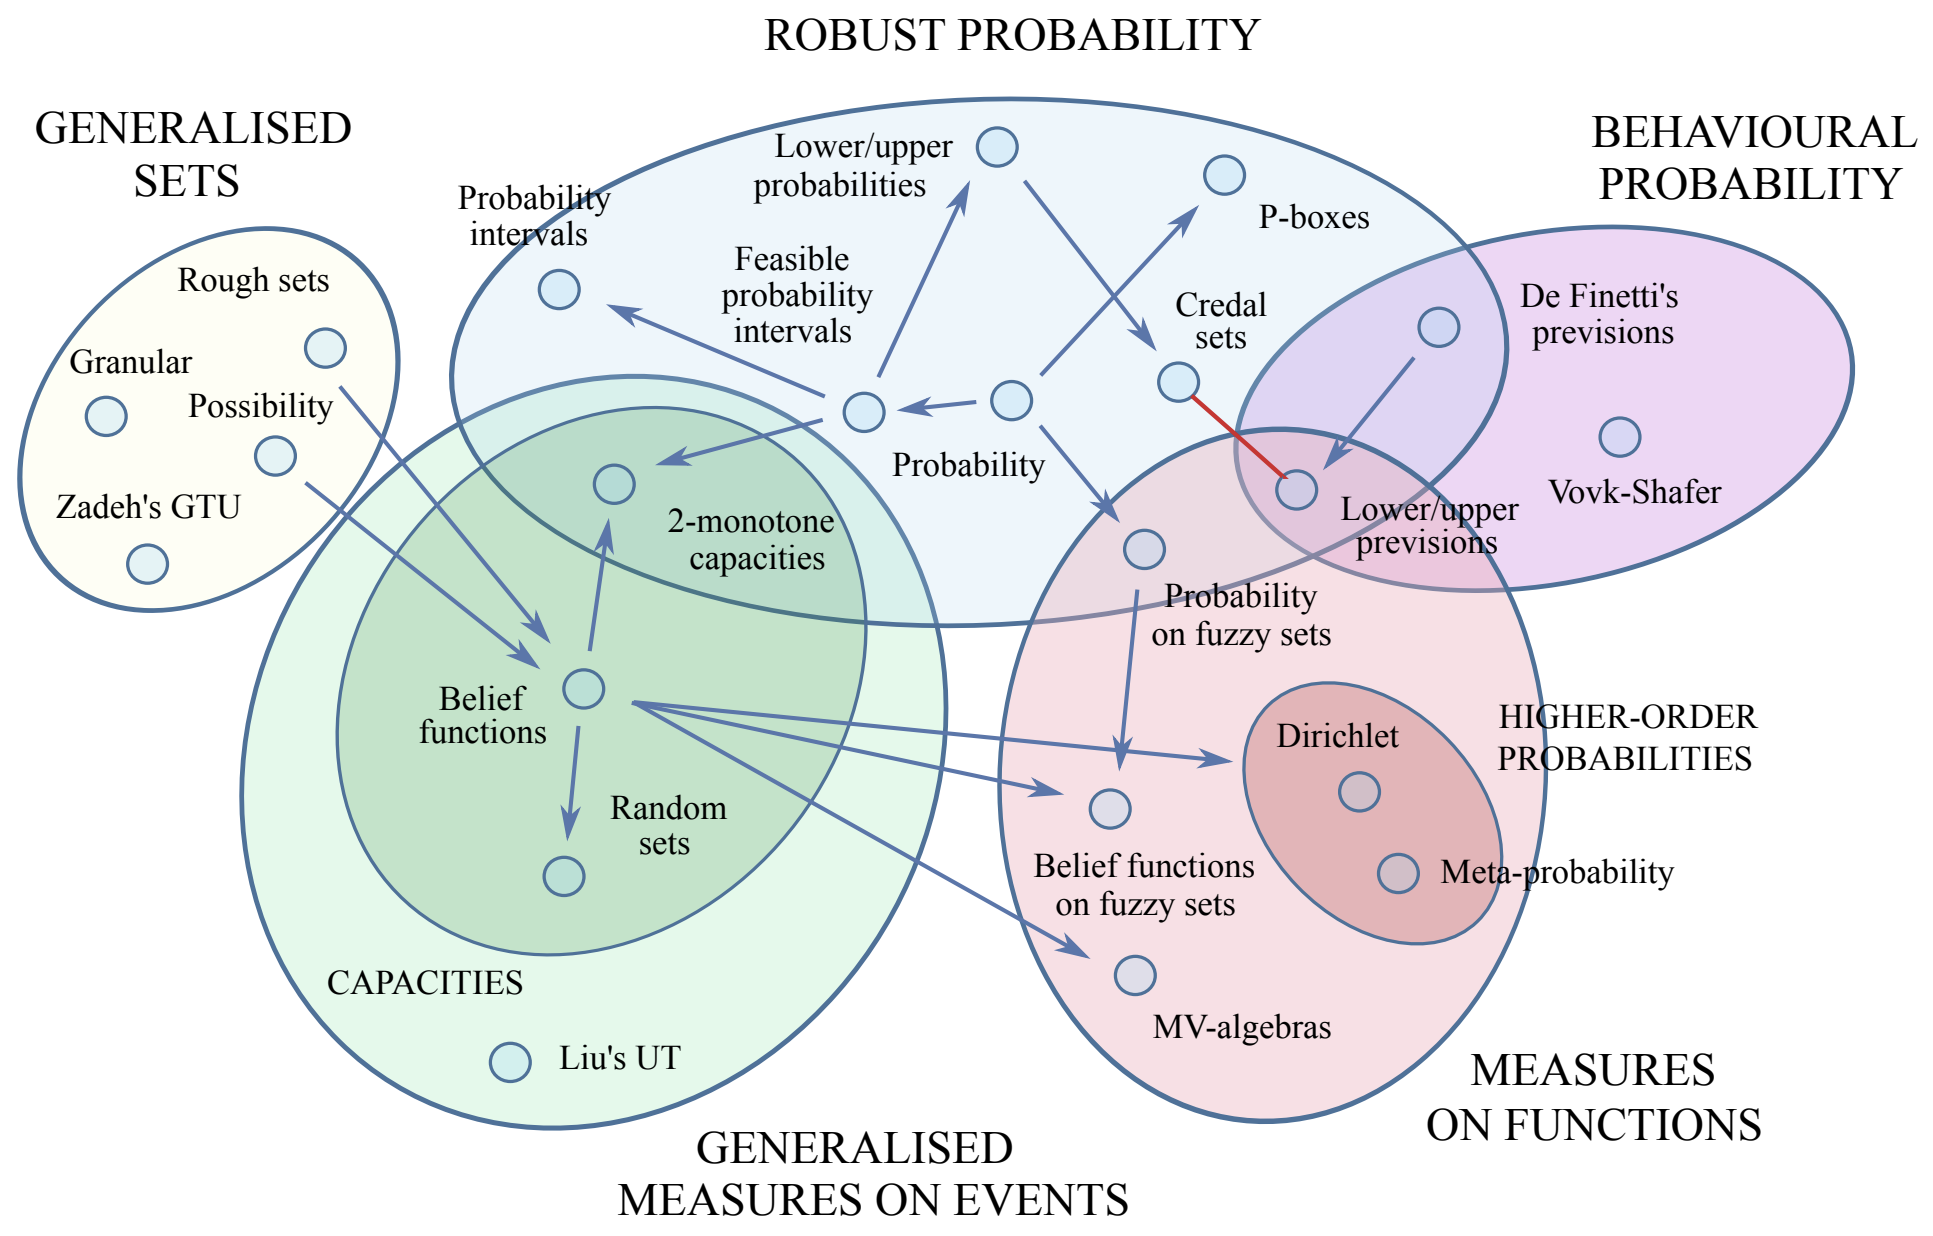
\includegraphics[width=\textwidth]{ch0/figures/Uncertainties Diagram.png}
    \caption{A classification of uncertainty theories showing their relationships and hierarchies. The theories are grouped based on their rationale and class of objects they attempt to mathematically model. Arrows indicate generalization relationships, pointing from more specific to more general frameworks. Extracted from \cite{uncertaintymeasuresbigpicture}.}
    \label{fig:uncertainty_taxonomy}
\end{figure}











































